\documentclass[a4paper,11pt,reqno]{amsart}

\pagestyle{headings}
\usepackage{graphicx}
\usepackage[english]{babel}
\usepackage[T1]{fontenc}
\usepackage[latin1]{inputenc}
\usepackage{verbatim}
\usepackage{amsmath}
\usepackage{amsfonts}
\usepackage{amssymb}
\usepackage{amsthm}
\usepackage{pstricks}
\usepackage{mathrsfs}
\usepackage{textcomp}
\usepackage{tikz}
\usepackage{subfig}
\usepackage{fancyvrb}
\usepackage{hyperref}

\title{\mbox{Bare-metal programming on the Raspberry Pi 2}}
\author{Didrik Lundberg\\
\texttt{didrikl@kth.se}}
\date{\today}
\begin{document}
\maketitle
\noindent
This is a comprehensive guide that will cover all steps of bare-metal programming necessary to run and debug the SICS Thin Hypervisor~\cite{do14sth} for the Raspberry Pi 2. Ubuntu 15.04 was used in the writing of this guide, but expect similar behaviour on similar systems. If you have any questions, please send an E-mail to the author.

Furthermore, I would like to thank Brian Sidebotham~\cite{sidebotham14guide} and David Welch~\cite{welch14guide} for their excellent guides for bare-metal programming on the Raspberry Pi 1 and 2.
\section{Introduction}
In order to follow this guide, you will need some equipment:
\begin{itemize}
  \item A Raspberry Pi 2 Model B single-board computer
  \item A PC to program on
  \item Internet connection via an Ethernet cable
  \item An SD card reader
  \item A serial-to-USB converter cable
  \item A USB to serial interface converter module (for JTAG)
   \begin{itemize}
    \item ... including the USB cable to connect it to your PC
  \end{itemize}
  \item For testing the hardware:
  \begin{itemize}
    \item A USB mouse and a USB keyboard
    \item A monitor with a HDMI cable connection
  \end{itemize}
\end{itemize}
Most items should be pretty straightforward to acquire. RPi2 uses micro-SD cards, so you will require your SD card reader to be able to read those. The serial port of the RPi2 is more specifically a UART using the 3.3V TTL standard of voltages - please note that converter cables which use other standards, such as RS-232, may fry your RPi2! However, some cables work for both RS-232 and 3.3V TTL. Look up the specifications of the chip in the converter cable you are buying just to be sure.

The UART communicates via two GPIO pins on the ordinary RPi2 pin block. However, the serial-to-USB converter cable should typically have four jumper wire connectors on one end and a USB connector on the other (the two additional wires providing ground and 5V power). If you find this to be confusing to sort it out yourself, I bought a serial-to-USB converter cable which uses the PL2303HX chip to transform the signal which I recommend - that chip name might be a good word to search the Internet for if you want to buy one yourself.

\section{Testing the equipment}
First, we must make sure that all our equipment is functional. To do this, we first download NOOBS from the homepage of the Raspberry Pi Foundation~\cite{noobs}. NOOBS is an operating systems installer, which we will use to comfortably set up Raspbian for testing purposes.

Simply format your SD card in the FAT32 file system (using for example \texttt{gparted}) and transfer the decompressed contents of the NOOBS folder to it, and you are ready to boot your RPi2 for the first time. Put your SD card in the RPi2, connect the Ethernet cable, the USB keyboard and mouse, the monitor, and then finally plug in the micro-USB cable (connected to your PC or to a USB power adapter of good quality on the other end) to supply power and your RPi2 will boot into NOOBS.

Install Raspbian, and inside Raspbian install the \texttt{screen} utility by typing \texttt{sudo apt-get install screen} in the terminal. Also install \texttt{screen} on the PC you are programming on in the same way.

Now it is time to connect the RPi2 to your computer with serial-to-USB converter cable. You must do this with great care, since connecting the wrong jumper wire to certain pins might fry your equipment. We will explain how to do this for our generic PL2303HX cable. It has four jumper wires:

\begin{itemize}
  \item \textbf{TxD}: Green. The ``T'' in the acronym stands for ``transmission'' - should be connected to the UART receiver pin (RxD) on the RPi2 block.
  \item \textbf{RxD}: White. The ``R'' in the acronym stands for ``receiving'' - should be connected to the UART transmission pin (TxD) on the RPi2 block.
  \item \textbf{Ground}: Black. Should be connected to the Ground pin on the RPi2 pin block.
  \item \textbf{5V power}: Red. WARNING! Do not plug this cable in if you are also supplying power via a micro-USB cable - that might fry the RPi2. This cable is an alternate way of providing power to the RPi2 without using a micro-USB cable.
\end{itemize}

It is important to note that the pin layout of the RPi2 is closely resembles that of other versions, the difference being that it has more pins (40 compared to 26 for the RPi). The 26 first pins counting from the pin closest to the SD card have the same functions. There are two ways of numbering the GPIO pins - using their GPIO numbers by which they are referred to by the computer, or using how they are physically ordered on the board, which might be a source of some confusion.
\begin{figure}[hb]
\begin{center}
   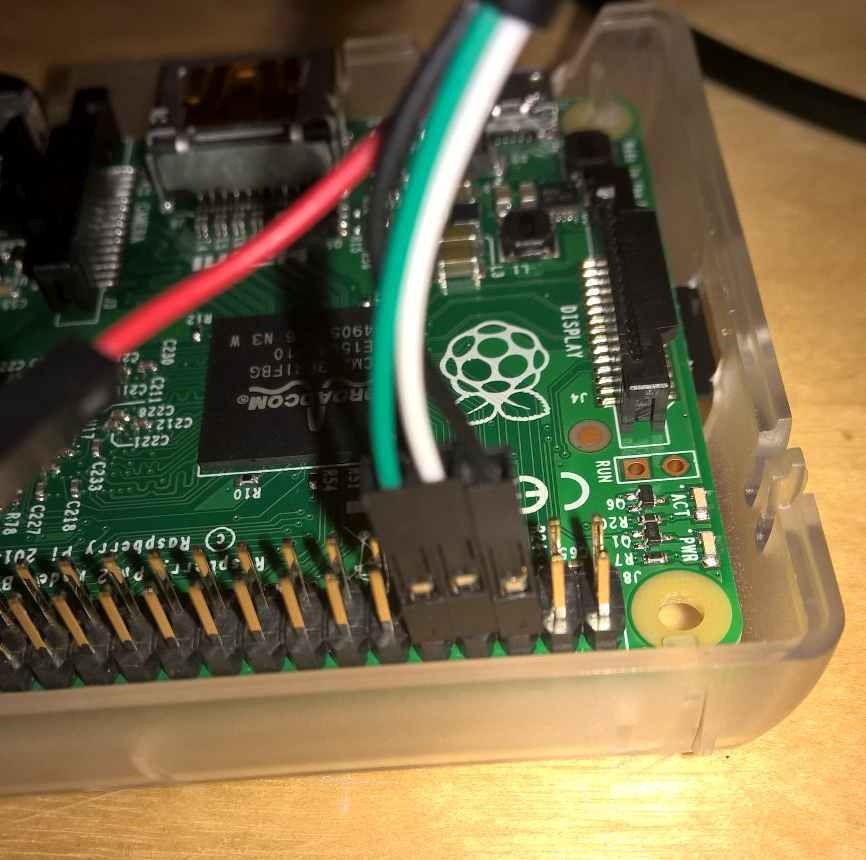
\includegraphics[scale=0.3]{connection.png}
 \end{center}
 \caption{The serial-to-USB converter as it looks connected to the RPi2}
 \label{fig:conn}
\end{figure}
\begin{figure}[hb]
\begin{center}
   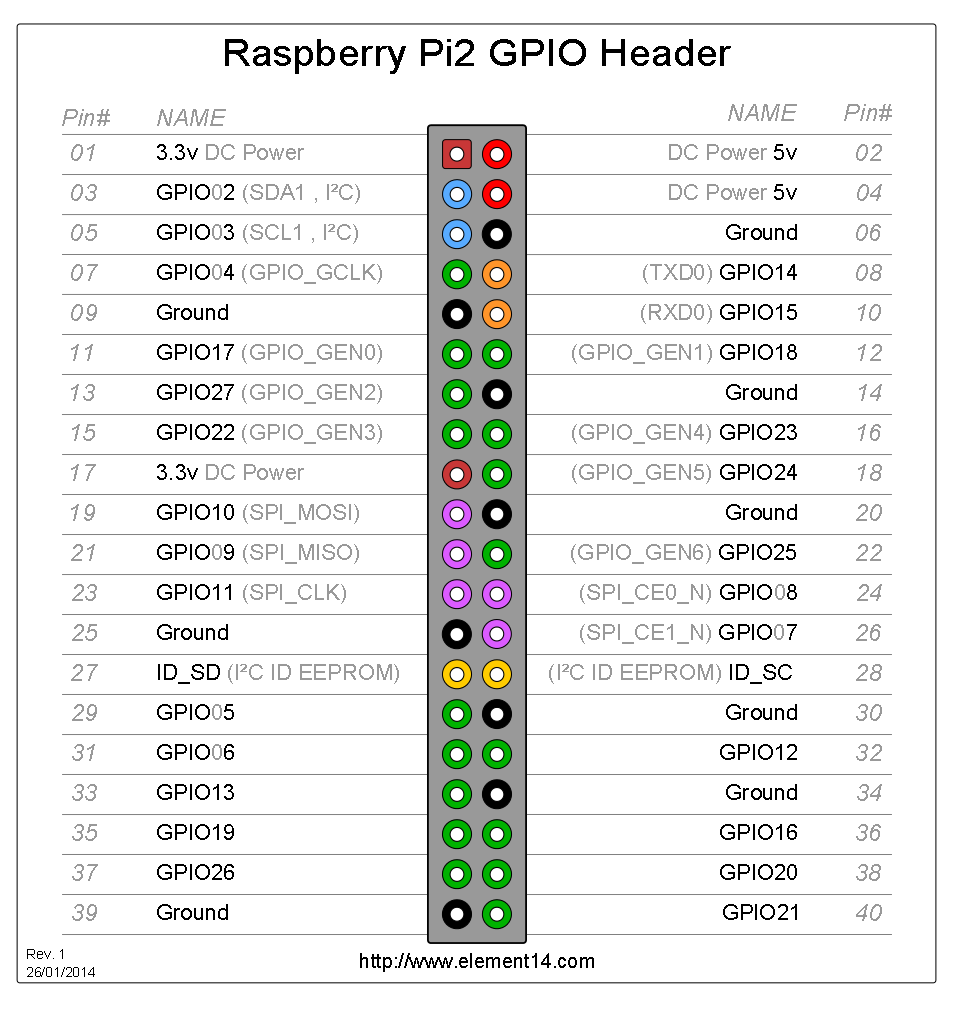
\includegraphics[scale=0.3]{GPIO_Pi2.png}
 \end{center}
 \caption{The RPi2 pin numbering}
 \label{fig:pins}
\end{figure}

So, by the above physical numbering seen in Figure~\ref{fig:pins}, the ground wire should be connected to pin 6, the receieve wire should be connected to pin 8, and the transmit wire to pin 10, as shown in Figure~\ref{fig:conn}. If you know what you are doing, you can also power the RPi2 by connecting the power wire to pin 2 or 4, but then you risk frying your equipment if you supply power over the micro-USB at the same time, so I would not recommend this.

Now, you first want to check that the serial-to-USB cable works correctly. To do this, write \texttt{lsusb} in a terminal window, and you should see a list of connected USB devices, in which the serial-to-USB cable should be identified. Second, we need to know the device name of the cable. Simply use \texttt{dmesg | grep usb} and you should be able to filter out the device name of the cable among the driver messages (in my case \texttt{/dev/ttyUSB0}).

Setting up the connection on the RPi2 should be easy - simply write \texttt{sudo screen /dev/ttyAMA0 115200}. The number at the end is the symbol rate of the connection, measured in bauds (bits per second). Similarly, on your computer, write \texttt{sudo screen /dev/ttyUSB0 115200}, where you replace the device name if needed. Now, if everything works correctly you should be able to write on the PC and see the characters appearing on the monitor connected to the RPi2, and vice versa. This ensures us that all the hardware works correctly, saving us valuable time looking for errors later if that should not be the case.

\section{Writing a test program}
Now, you will need an empty SD card. Either re-format the one you have, again to FAT-32, or use another one, which might be more handy if you need Raspbian later on.

Writing a bare-metal program requires intimate knowledge about the hardware. The hardware of the RPi2 is very similar to that of the RPi, whose chip BCM2835 has excellent documentation~\cite{bcm2835}. The only significant difference is the processor, and the increased RAM of the RPi2. Indeed, there are more differences, such as for example a mini-UART which is not on the RPi2, but these differences are not relevant for this guide.

It follows that we can use the BCM2835 documentation for working with the RPi2, with a few important corrections: the base address of the peripherals has changed from \texttt{0x20000000} to \texttt{0x3F000000}, and the memory bus address offset \texttt{0x40000000} has changed to \texttt{0xC0000000}. Accordingly, all addresses you read in the documentation will have to be adjusted with this in mind. Typically, this just means that you replace \texttt{20} at the start of a hexadecimal number with \texttt{3F}. The rest of the changes between BCM2835 and BCM2836 are processor-related.

Technically speaking, we are going to write a kernel - although our ``kernel'' will not have much of the functionality we associate with one, it will take the place of a kernel during the boot process. It follows that we require a bootloader and other accessories to get running. The easiest way to solve this is to obtain the GitHub repository \texttt{raspberrypi/firmware} and copy the contents of the \texttt{boot} folder to your SD card, deleting the files \texttt{kernel.img} and \texttt{kernel7.img} (which are the existing kernels). We end up with some redundant files, but are guaranteed things will work.

\subsection{Setting up a cross-compiler}
You will require a compiler which can compile code to run on other hardware. This is easily solved by the GNU ARM Embedded Toolchain, which is installed by the command \texttt{sudo apt-get install gcc-arm-none-eabi} and you are good to go. Then, to compile \texttt{test.c}, you would use \texttt{arm-none-eabi-gcc -O2 -mfpu=vfp -mfloat-abi=hard -march=armv7-a -mtune=cortex-a7 -nostartfiles test.c -o kernel.elf}. However, we do not want an ELF file, but a binary which only includes machine code, so we extract that part from \texttt{kernel.elf} using the \texttt{objcopy} utility: \texttt{arm-none-eabi-objcopy kernel.elf -O binary kernel.img}, and get the binary we want in \texttt{kernel.img}. This can then be put on the SD card together with the bootloader, as described above, which will look for the kernel.img and execute it.

\subsection{Setting up CMake}
However, in reality we never just compile a single C file. We are going to have multiple files in C and ARM assembly language and so we will need CMake, in order to keep things neat and tidy. To install CMake, execute the command \texttt{sudo apt-get install cmake}. Now, the CMake-related files you start out with are \texttt{CMakeLists.txt}, \texttt{configure.sh}, and \texttt{toolchain-arm-none-eabi.cmake}. These are fairly self-explanatory, but you should know that you will need to change them if you change the structure of your project (add more files, change names of files, and so on). Otherwise, all you need to know is that you set up CMake by executing \texttt{./configure.sh}, and then build simply with \texttt{make}. 

\subsection{Example code}
Several useful example programs (or ``test kernels'') can be found in the GitHub repository \texttt{guancio/kth-on-rpi2}, in the \texttt{rpi2-port} directory. These consists of code in C, ARM assembly language, and a linker file called \texttt{linker.ld}

The linker script decides where to physically put different parts of the code in the binary file, for example the magic number we want in order to pose as a Linux kernel when using U-Boot. If you change the linker script or the assembly code in \texttt{boot.S}, make sure that the magic number is in the correct position if you are using U-Boot as described below (this can easily be ensured by adding new sections for your own code in \texttt{boot.S} and inserting them after \text{.magic} in the linker script).

A more thorough description of the C and assembly code of these test kernels can be found in the comments inside the files, please also keep the BCM2835 documentation as a reading companion.

\subsubsection{test-kernel-1}
This test kernel will make the green LED on the RPi2 blink, with approximately one-second intervals between each flash. This simple program is good for testing if your pipeline to get code running on the RPi2 is working correctly.

\subsubsection{test-kernel-2}
This test kernel will blink and write alternately ``Hello, Kernel World!'' and ``Goodbye, Kernel World!'' over the UART in perpetuity, with approximately one second of waiting in between each output. This is useful for testing serial connection over the UART.

\subsubsection{test-kernel-3}
This test kernel will first setup certain pins on the RPi2 for JTAG communication, and then blink and write alternately ``Hello, kernel world!'' and ``Goodbye, kernel world!'' over the UART in perpetuity, with approximately two seconds of waiting in between each output. This is useful for testing both JTAG and serial connection.

\section{Booting over a network}
Start by downloading the GitHub repository \texttt{raspberrypi/firmware} (if you do not already have it downloaded) and copy the contents of the \texttt{boot} folder to your SD card, as described before. Then, open the file \texttt{config.txt} on your SD card, and change it to read \texttt{kernel=u-boot.bin}, instead of where \texttt{kernel} pointed to before.

Next, you will need to create a script that U-Boot will run once it is started. Create a file called \texttt{boot.scr}, and enter the following:

\begin{figure}[hb]
\begin{center}
\begin{BVerbatim}
usb start
setenv scriptaddr 0x02000000
setenv serverip 130.229.149.236
setenv ipaddr 130.237.224.169
setenv bootargs "console=tty0"
tftp ${kernel_addr_r} zImage
bootz ${kernel_addr_r}
\end{BVerbatim}
\end{center}
\caption{Boot script for U-Boot}
\label{fig:boots}
\end{figure}

where you replace the IP address after \texttt{serverip} by the one of your computer (which will act as a TFTP server later on). Your IP address can be found by looking at your \texttt{inet addr} after executing the \texttt{ifconfig} command in a terminal window.

Also replace the IP address after \texttt{ipaddr} in the boot script by an address belonging to your local network which is currently unoccupied - this will be the IP address of the RPi2. As a strategy, choose an address close to yours (alter only numbers near the right end of the IP) and ping it, using the command \texttt{ping 130.237.224.169}, where you replace the IP address with the one you want as the IP address of your device.

It might also be worth noting that \texttt{usb start} scans bus 0 for storage and Ethernet devices, which include your Ethernet port. Without this line, you will not be able to connect to your computer via TFTP. The \texttt{scriptaddr} is explicitly defined in the script for pedagogic reasons. This might not be needed, but you need to remember to not overwrite U-Boot on memory with the boot script. 

This bootscript presupposes that you have a monitor connected to the RPi2 via a HDMI cable. If you instead rely on serial connection to see what is happening (not recommended at this point), you should replace \texttt{console=tty0} with \texttt{console=ttyAMA0} (or simply use both). Bootargs usually also sets properties of the file system, but since we are not using it in our trivial examples, it is not needed here.

Now that we have written the bootscript, we want to convert it to an image. Do this by executing the command \texttt{mkimage -A arm -O linux -T script -C none -n Boot Script -d boot.scr boot.scr.uimg}. The result will be stored in \texttt{boot.scr.uimg} - transfer this file to your SD card.

Now we only have one part left - U-Boot itself. First, we have to download U-Boot. Download it by executing the command \texttt{git clone git://git.denx.de/u-boot.git
}, which will create U-Boot to a directory at your current location. After that is done, we get the required cross-compiler by \texttt{apt-get install gcc-arm-linux-gnueabihf}. Also install U-Boot tools with \texttt{apt-get install u-boot-tools}. Now open a terminal window in the folder you have U-Boot in, and execute the command \texttt{make rpi\_2\_defconfig}, followed by \texttt{make all -j8}. After the build is finished, copy all files starting with \texttt{u-boot} to your SD card. Now, you can eject your SD card and place it in your RPi2.

We are now going to set up your computer as a TFTP server. First, we install the required tools by executing the command \texttt{sudo apt-get install xinetd tftpd tftp}. Edit (or create, if it does not exist) \texttt{tftp} in \texttt{etc/xinet.d/}, which should contain the following:

\begin{figure}[hb]
\begin{center}
\begin{BVerbatim}
service tftp
{
    protocol        = udp
    port            = 69
    socket_type     = dgram
    wait            = yes
    user            = nobody
    server          = /usr/sbin/in.tftpd
    server_args     = /tftpboot
    disable         = no
}
\end{BVerbatim}
\end{center}
\caption{TFTP server configuration}
\label{fig:server}
\end{figure}

Then, create a directory called \texttt{tftpboot} in \texttt{/}. Make sure you do not have too stingy access rights by executing the commands \texttt{sudo chmod -R 777 /tftpboot} and \texttt{sudo chown -R nobody /tftpboot} in the directory where you created \texttt{tftpboot}. Then, make your changes take effect by executing \texttt{sudo service xinetd restart}.

Now, we need to prepare the kernel in question we want to remote boot. The boot script requires us to trick bootz into believeing it has received a Linux kernel. To do this, we must insert a so-called ``magic number'' \texttt{0x016F2818} into the code. Here, you will need a hex editor to verify what you are doing. Get one with the command \texttt{sudo apt-get install bless}. Enter the \texttt{boot.S} (or whatever the ARM assembler part of your kernel is named) and declare a dummy variable (with no name) by inserting the line \texttt{.word 0x016f2818} outside of a function. Compile the kernel, and then search for ``18286F01'' in the image file (not the ELF file) using the hex editor. These bytes should be found starting at the offset \texttt{0x24}. If they are at a higher offset in the program, move the declaration up in the \texttt{boot.S} file. If the bytes are found at a too low offset, declare more dummy variables (\texttt{.word 0x01010101}, and so on...) before the magic number until you can find it at the correct offset. Finally, when this is done, rename your kernel \texttt{zImage} and move it to the \texttt{tftpboot} directory.

The setup is now complete. Plug in an Ethernet cable and a HDMI cable connected to a monitor to your RPi2 and power it from micro-USB to observe your program booting from U-Boot.

If at any point you should shut down your computer, you will need to start the server again by writing \texttt{sudo /etc/init.d/xinetd restart}, and take a second look if the IP addresses in your boot script can still be used; otherwise you will need to change the bootscript, create the boot script image again, and transfer it to the SD card.

\section{Setting up JTAG}
Communicating over JTAG with you PC can be very useful when debugging code on an external device. We will therefore look into the matter of using a JTAG adapter for this purpose. In this guide, we will be using a FT2232H Mini-Module~\cite{ft2232h}~\cite{ft2232hmm}, which is very cheap, fast, and allows us to communicate both over UART and JTAG at the same time using only one adapter.

First, we need to be sure that the hardware is working. The FT2232H Mini-Module has two pin blocks, which are distinguished by their names ``CN2'' and ``CN3'' (channel 2 and channel 3, respectively) which can be found at the edge of the pin blocks on both sides of the board. The pins on the blocks are physically numbered starting from the pin marked by a square on one side of the board as pin 1, the pin which is on the same row of two as pin 1 being pin 2, and so on. So one of the two long rows of the pin blocks consists of odd numbers, and vice versa.

The adapter is not powered unless you make some connections between the pins on the board itself. For this purpose, you will need to use jumper cables.

\begin{figure}[hb]
\begin{center}
\begin{itemize}
\item VBUS to VCC:
		\begin{itemize}
		\item CN3-1 to CN3-3
		\end{itemize}
\item V3V3 to VIO:
		\begin{itemize}
		\item CN2-1 to CN2-11
		\item CN2-3 to CN3-12
		\item CN2-5 to CN2-21
		\item CN2-9 to CN2-10
		\end{itemize}
\end{itemize}
\end{center}
\caption{Trivial jumper cable connections}
\label{fig:con1}
\end{figure}

Connect jumper cables between the pins as described in the list above, and then plug a mini-USB cable into the adapter on one end and your PC on the other end. At this point, you should be able to find the adapter listed when using \texttt{lsusb} and the two different device names of the different channels when using \texttt{dmesg | grep usb} (using the connections above, \texttt{/dev/tty0} for the JTAG and \texttt{/dev/tty1} for UART).

When you have verified that the above works, disconnect the adapter from its power source and set up the cabling described below.

\begin{figure}[hb]
\begin{center}
\begin{itemize}
	\item JTAG: (FT2232H board left, RPi2 right)
		\begin{itemize}
		\item TCK:   CN2-7   to 22 (GPIO number 25)
		\item TDI:   CN2-10  to 7 (GPIO number 4)
		\item TDO:   CN2-9   to 18 (GPIO number 24)
		\item TMS:   CN2-12  to 13 (GPIO number 27)
		\end{itemize}
	\item UART:
		\begin{itemize}
		\item TXRX:  CN3-26  to 10 (GPIO number 15)
		\item RXTX:  CN3-25  to 8 (GPIO number 14)
		\end{itemize}
	\item Ground:
		\begin{itemize}
		\item GND:   CN2-2   to 6
		\end{itemize}
	\item RPi2 to RPi2:
		\begin{itemize}
		\item V3V3 to TRST:  1    to 15 (GPIO number 22)
		\end{itemize}
	\item FTDI board to FTDI board:
		\begin{itemize}
		\item V3V3 to VCCIO: CN2-1   to CN2-11
		\item VBUS to VCC:   CN3-1   to CN3-3
		\end{itemize}
\end{itemize}
\end{center}
\caption{JTAG and UART jumper cable connections}
\label{fig:con2}
\end{figure}
\begin{figure}[hb]
\begin{center}
   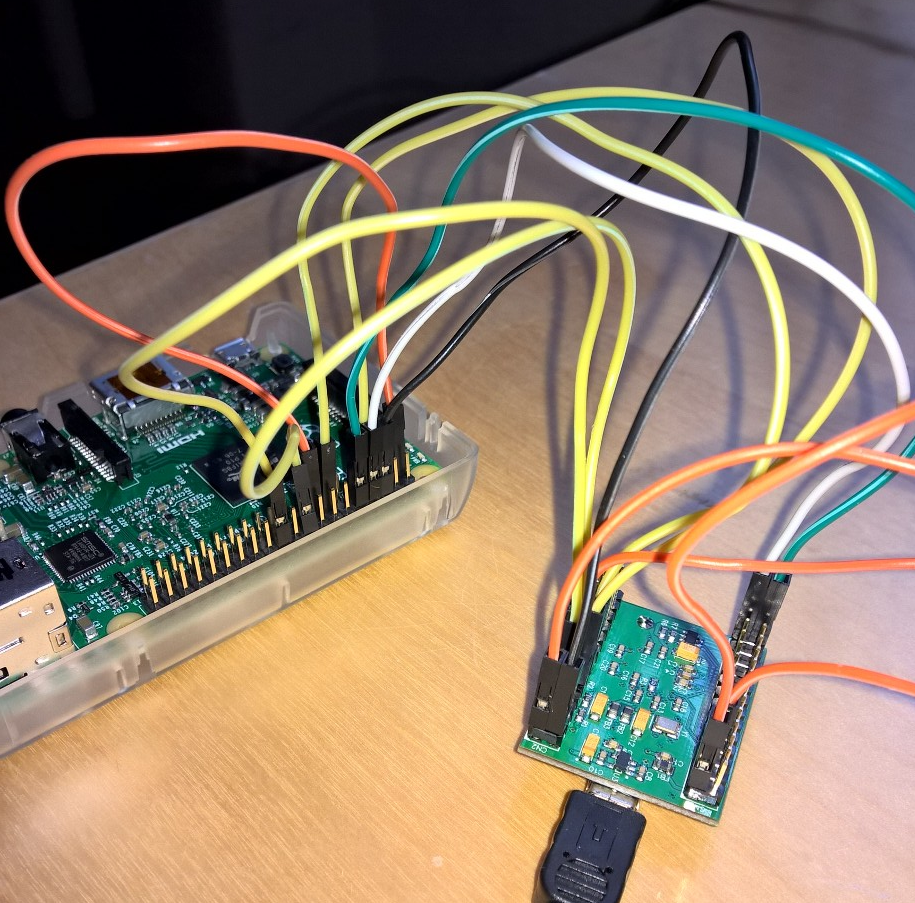
\includegraphics[scale=0.3]{connection2.png}
 \end{center}
 \caption{The FT2232H Mini-Module as it looks connected to the RPi2 via both JTAG (yellow cables), ground (black cable) and the UART (green and white cable)}
 \label{fig:conn2}
\end{figure}

If you happen to have a FT4232H Mini-Module instead, the connections at this point are identical except for the UART, where you would instead connect pins 8 and 10 on the RPi2 to the CN2-17 and the CN2-18 pins on the adapter, respectively. I have also listed the GPIO number of the RPi2 pins.

Next, before we plug this in, we need to install the software we need. To communicate over UART, we will simply use the tools we used before (\texttt{screen} or \texttt{minicom}). To communicate over JTAG, we will need the latest version of OpenOCD. For following this guide, we recommend at least version 0.9.0. In general, for getting the latest version of this tool, I recommend cloning the OpenOCD Git repository. First, you need to acquire some dependencies. Do so by executing the command \texttt{sudo apt-get install make libtool pkg-config autoconf automake texinfo}.

You can use either FTDI's own drivers (ftd2xx) or the open-source driver library libFTDI. At some point in time, the ftd2xx driver was much faster, although the issues with using it consists of not being able to redistribute your compiled code. Currently, I think they are about as fast and so it is more convenient for us to use libFTDI. Install libFTDI by executing the command \texttt{sudo apt-get install libusb-1.0-0-dev}.

Now clone the OpenOCD Git repository by executing the command \texttt{git clone git://git.code.sf.net/p/openocd/code}. Navigate to the directory where OpenOCD was cloned, and type \texttt{./configure --enable-ftdi}, which should do the trick for configuration.s Then type \texttt{make} (make sure there are no errors!) and then \texttt{sudo make install}.

OpenOCD is now installed! Now, you need to run it. For this, you will need two configuration files. One for the JTAG adapter and one for the SoC board. In other words, use something similar to:

\begin{verbatim}
openocd -f interface/ADAPTER.cfg -f target/MYTARGET.cfg
\end{verbatim}

where you replace \texttt{interface/ADAPTER.cfg} and \texttt{target/MYTARGET.cfg} with the corresponding files for your JTAG adapter and the board you want to debug on. In our case this becomes

\begin{verbatim}
openocd -f interface/ftdi/minimodule.cfg -f target/raspberrypi2.cfg
\end{verbatim}

You might not have a file for the RPi2 on your OpenOCD installation, though. If you do not, you must create one. The installed OpenOCD scripts are stored at \texttt{/usr/local/share/OpenOCD/scripts}. To easily create new files, execute the command \texttt{gksudo thunar}, and use the Thunar graphical file manager to navigate the the directory of the scripts and create and modify files there. Specifically for the RPi2 script, create a new file containing the Tcl code found at \texttt{rpi2-port/raspberrypi2.cfg}, in the \texttt{guancio/kth-on-rpi2} GitHub repository.

Now, you will need to write a kernel which enables the pins you have connected your JTAG adapter for JTAG communication. One such example, which can be used with U-Boot as described above, can be found in the GitHub repository \texttt{guancio/kth-on-rpi2}, in the \texttt{rpi2-port} folder, named \texttt{test-kernel-3}. Start your RPi2 as described in the U-Boot section above (or use the test kernel \texttt{test-kernel-3-standalone} instead if you do not want U-Boot), and plug the USB cable connected to your FT2232H Mini-Module into your computer. You must then wait for the pins to be enabled for JTAG use. You can tell this is the case when the green ``OK'' LED is blinking with two-second intervals. Then, execute the command

\begin{verbatim}
openocd -f interface/ftdi/minimodule.cfg -f target/raspberrypi2.cfg
\end{verbatim}

Your OpenOCD should now detect the processor of your debug target. It will list the number of processors, and their respective breakpoints and so on, and then wait. At this point, you want to open a new terminal window and connect to OpenOCD, for example by executing the command \texttt{telnet localhost 4444} to communicate via Telnet. That will put you in communication with OpenOCD and you will be able to execute a number of commands in that environment. First, try the command \texttt{help} to see what you can do. For a simple test, you can execute the command \texttt{targets} followed by \texttt{halt} and then \texttt{targets} again to verify that you can use JTAG. Execute the command \texttt{exit} to exit the Telnet connection.

Now, we also want to be able to communicate via UART at the same time. At some point before you connect to OpenOCD and halt the processors (if you have already done this, shut down OpenOCD and remove power from your RPi2, then connect to power and re-connect OpenOCD as described above), you can connect to one of the channels of the adapter. Use \texttt{dmesg | grep usb} and look for lines which say \texttt{FTDI USB Serial Device converter now attached to ttyUSBX}, where \texttt{X} is an integer. If you have connected OpenOCD, you will see that one of these have been disconnected - that is where the adapter communicates via JTAG with OpenOCD. Connect to the remaining one using \texttt{sudo screen /dev/ttyUSBY 115200}, where \texttt{Y} is the number of the remaining connection. Using any of the test kernels described in this section, you should see the lines ``Hello, kernel world!'' and ``Goodbye, kernel world!'' printed alternately in perpetuity.

\bibliography{Guide}{}
\bibliographystyle{acm}
\end{document}
